\documentclass[12pt, onecolumn]{article}

\usepackage[portuguese]{babel}
\usepackage[latin1]{inputenc}
\usepackage[T1]{fontenc}
\usepackage[cm]{fullpage}
\usepackage{hyperref}
\usepackage{graphicx}
\usepackage{float}

\title{Universidade de Coimbra \\
Departamento de Engenharia Inform\'atica\\
Computa\c{c}\~ao Gr\'afica\\
Projeto - Jogo do Galo em Primeira Pessoa}


\date{}

\begin{document}

\clearpage\maketitle
\thispagestyle{empty}
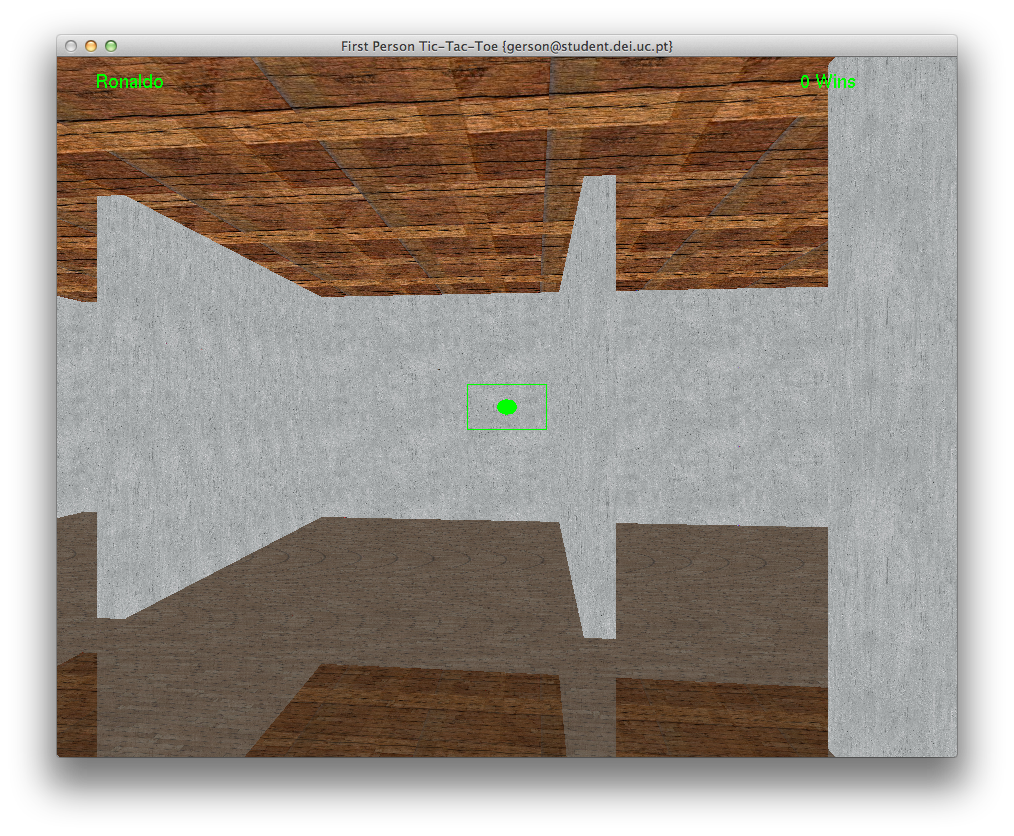
\includegraphics[scale=0.5]{game.png}
\vfill
\begin{center}
  {\Large Coimbra, \today}
\end{center}

\newpage\tableofcontents

\twocolumn

\section{Elemento do Grupo}

\paragraph{G\'erson de Paulo Carlos} 
\begin{itemize}
  \item{N$^{o}$:} 2012163742 
  \item{Email:} \href{mailto:gerson@student.dei.uc.pt}{gerson@student.dei.uc.pt}
  \item{Turma:} PL4
  \item{Tempo de esfor\c{c}o:} 75 horas
  \item{Tarefas cumpridas:}
  \begin{itemize}
    \item Implementa\c{c}\~ao
    \item Testes
    \item Relat\'orio
  \end{itemize}
\end{itemize}


\section{Introdu\c{c}\~ao}

O projeto buscou aplicar os conhecimentos adquiridos durante todo o semestre de uma forma mais interessante, implementando uma vers\~ao do \textbf{Jogo do Galo} em 3D, aplicando algumas das t\'ecnicas aprendidas.

O relat\'orio est\'a seccionado da seguinte forma. Primeiramente, s\~ao apresentadas as principais caracter\'isticas implementadas no projeto. Posteriormente, s\~ao fornecidos alguns detalhes pertinentes \`a implementa\c{c}\~ao. Em seguida, s\~ao apresentados os controles de intera\c{c}\~ao com o utilizador. E por \'ultimo uma breve conclus\~ao do projeto.


\section{Features}

Destaca-se aqui as principais caracter\'isticas que foram implementadas no projeto.

\subsection{Transforma\c{c}\~oes}

Foram utilizadas para poder mover algumas partes do cen\'ario, como o HUD e as figuras O e X. A vis\~ao do jogador \'e alterada atrav\'es da correta mudan\c{c}a da posi\c{c}\~ao da c\^amera pelo \texttt{Viewport}.

\subsection{Proje\c{c}\~oes}

Com o uso diversificado das proje\c{c}\~oes ortogonal e paralela, criou-se duas vis\~oes principais: a 3D, em primeira pessoa; e a superior, indicando como que uma mapa do jogo atual.

\subsection{Ilumina\c{c}\~ao}

Foi utilizado uma ilumina\c{c}\~ao ambiente vari\'avel, podendo ser setada pelo utilizador no menu popup o n\'ivel de intensidade.

\subsection{Nevoeiro}

H\'a op\c{c}\~ao para o jogador de adicionar o nevoeiro \`a cena do jogo. Por padr\~ao, o jogo come\c{c}a sem nevoeiro algum e atrav\'es do menu popup o jogador pode iniciar um jogo ainda com um nevoeiro fraco ou nevoeiro forte, o que vai acabar colocando a vari\'avel \texttt{fog\_density} para o valor apropriado.

\subsection{Texturas}

Com o apoio da biblioteca \texttt{RgbImage}, utilizou-se texturas nas paredes, no ch\~ao e no teto para tornar a cena do jogo mais interessante. Para otimizar um pouco o processamento necess\'ario, atrav\'es de \texttt{glCullFace} para descartar do pipeline os pol\'igonos que n\~ao t\^em a face frontal vis\'ivel.

\subsection{Reflex\~ao}

A partir do c\'odigo disponibilizado no \textit{inforestudante}, utilizando \texttt{STENCIL BUFFER}, adicionou-se uma reflex\~ao no ch\~ao da cena, aumentando um pouco o realismo.

\twocolumn

\section{Implementa\c{c}\~ao}

O projeto foi implementado todo em C++ e o c\'odigo foi separado em dois conjuntos de arquivos: \texttt{main.cpp}/\texttt{main.h} e \texttt{extra.cpp}/\texttt{extra.h}, buscando deixar organizado um projeto de consider\'avel tamanho.

Foram criadas classes auxiliares \texttt{CFigure}, \break \texttt{CBall:CFigure} e \texttt{CExe:CFigure} para representar as figuras de jogo O e X; A classe \texttt{CWall} para representar cada uma das paredes internas; E a classe \texttt{CPlayer} para representar cada um dos jogadores. Futuramente, uma mais profunda utiliza\c{c}\~ao de classes deixaria ainda melhor o c\'odigo do projeto.

Quanto ao OpenGL, foram utilizadas as tr\^es bibliotecas b\'asicas apresentadas em aula: \texttt{gl}, \texttt{glu} e \texttt{glut}. Ainda foi utilizada a biblioteca \texttt{RgbImage} para a importa\c{c}\~ao de imagens a ser utilizadas para texturas.

Implementa\c{c}\~ao e testes em um Mac OSX 10.8.4.

\section{Controles}

Nesta se\c{c}\~ao s\~ao explicados os controles disponibilizados para o utilizador. Ao clicar com o bot\~ao direito do mouse, um menu popup \'e oferecido para o utilizador com op\c{c}\~oes para um novo jogo, altera a luz ambiente ou sair do jogo.

\subsection{Andar}
\begin{description}
  \item[W] andar para frente.
  \item[S] andar para tr\'as.
  \item[A] andar para a esquerda.
  \item[D] andar para a direita.
\end{description}

\subsection{Olhar}
\begin{description}
  \item[Mouse \`a direita] rodar no sentido hor\'ario.
  \item[Mouse \`a esquerda] rodar no sentido anti-hor\'ario.
\end{description}

\subsection{Marcar}
\begin{description}
  \item[Clique bot\~ao direito] marcar O ou X na posi\c{c}\~ao atual.
\end{description}

\subsection{Visualiza\c{c}\~ao do Mapa}

\begin{description}
  \item[M] Troca entre visualia\c{c}\~ao superior e vis\~ao em primeira pessoa.
\end{description}

\section{Conclus\~ao}

Este trabalho apresentou o desafio de criar uma aplica\c{c}\~ao para o Jogo do Galo, utilizando as t\'ecnicas de Computa\c{c}\~ao Gr\'afica aprendidas. Assim, com base na ideia de jogos de tiro em primeira pessoa (FPS), criou-se o jogo descrito, que fornece a possibilidade de realmente jogar o Jogo do Galo com as regras convencionais.

\end{document}
